\q{18}{HA/Biness Among Countries} \\ 

We are interesting in studying the distribution of human happiness across the world. To do so, we have a table called {\tt happiness}. The table has 140 rows, and the first few rows are shown below: 

\begin{center}
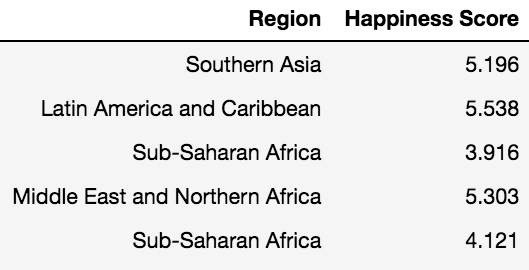
\includegraphics[scale=1]{countries.png}
\end{center}\\
\\ 
Each row contains the region and happiness score for a sampled country. The countries are not shown in the table above. Throughout this question, our goal will be to measure if the distribution of happiness scores across regions in the whole world are roughly equivalent. 

\begin{enumerate}
\subq{2} Define a function {\tt region\_happiness} which takes in a table like  {\tt happiness} and returns a two column table. The output table should have one column with the names of the unique regions, and a second column with the average happiness score in that region. The first few rows of an output table are shown below, with one row for each unique region. Note that the input table may not have the same labels as {\tt happiness}, but will have the same ordering of columns.

\begin{center}
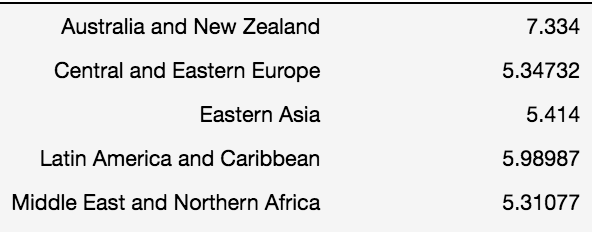
\includegraphics[scale=0.9]{regions.png}
\end{center}\\ \\ \\
 
\lstinline{def region_happiness(tbl):}\\ \\
\lstinline{     return ____________________________________________________________________________}
\\
\solution{
\lstinline{def region_happiness(tbl):}\\ \\
\lstinline{     return tbl.group(0, np.average)}}

We are in an abnormal situation, in which we have 10 different regions and we are interested in figuring out if the numerical distributions of all of the regions happiness scores are roughly equivalent. To do this, we will use a variant of A/B testing called multivariate testing. The only difference between the two methods is we have more than two groups (in this case, 10), and we are comparing the numerical distributions of all of these groups at the same time. 
\\ \\
The important thing to notice is that our null hypothesis and alternative hypotheses retain the same structure as they have for A/B testing, as well as our method for simulating a sample under the null. The only difference will be the test statistic we decide to use to differentiate between our two viewpoints. 
\\ \\
We are interested in testing if the distributions of happiness scores of all the regions come from the same underlying population distribution or not using our sample we have above.\\

\newpage
\subq{4}  Describe a specific null and alternative hypothesis that will help us pick between the two viewpoints presented above.\\ \\
\textbf{Null:} \\ \\ \\ \\
\textbf{Alternative:} \\ \\ \\
\solution{Null: The distributions of happiness scores for all regions are sampled from the same population distribution. Any difference in our sample is due to chance. \\
Alternative: The distributions of happiness scores for all regions do not come from the same population distribution. }
\subq{2} To help us differentiate between our two hypotheses, we need to choose a test statistic. Choose the best test statistic and corresponding explanation. 
\begin{itemize}[label = \bubble]
\item We should choose the TVD between the average happiness of each region and the expected average happiness of each region as our test statistic because only small values of our test statistic will point to the alternative hypothesis.
\item We should choose the TVD between the average happiness of each region and the expected average happiness of each region as our test statistic because only large values of our test statistic will point to the null hypothesis.
\item We should choose the standard deviation of the average happiness per region as our test statistic because only large values of our test statistic will point to the alternative hypothesis. 
\item We should choose the standard deviation of the average happiness per region as our test statistic because only small values of our test statistic will point to the alternative hypothesis. 
\item We should choose the median of the average happiness per region as our test statistic because only large values of our test statistic will point to the alternative hypothesis.
\end{itemize}
\solution{Option 3 -- standard deviation finds the overall variation from the average. If the null was true, each average human happiness score would be close to each other so our standard deviation would be low. If the alternative was true, the averages happiness will be further apart, and result in a large standard deviation. \\ \\
TVD does not work because we do not have any expected distribution of happiness scores. If the option talked about proportions of of happiness, then that would work, but notice that if you try to code some expected distribution of happiness score in the next question, you would be at an impass. }
\vfill
\subq{2} Define a function {\tt test\_statistic} which takes in a table like {\tt happiness} and returns the test statistic you chose from the last question. Note that the input table will not have the same labels, but will have the same ordering of columns. 
\\ 
You may use your {\tt region\_happiness} function from above and assume it is fully correct. \\

\lstinline{def test_statistic(tbl):} \\ \\
\lstinline{     regions = _________________________________________________________________________} \\ \\
\lstinline{     return ___________________________________________________________________________} \\
\solution{\lstinline{def test_statistic(tbl):} \\ \\
\lstinline{ regions = region_happiness(tbl)} \\ \\
\lstinline{ return np.std(regions.column(1))} }
\vfill
\subq{3}  Complete the definition of {\tt sample\_under\_null}, which takes in no arguments and returns one value of the test statistic applied to a random sample simulated under the null hypothesis. 
\\
You may use your {\tt test\_statistic} function from above and assume it is fully correct. 
\\

\lstinline{def sample_under_null():} \\ \\
\lstinline{     shuffled_hap = happiness.______________________________________________________________} \\ \\
\lstinline{     r_and_h = Table().with_column(________________________________________________________)} \\ \\
\lstinline{     return _________________________________________________________________________________} \\ \\
\solution{\lstinline{def sample_under_null():} \\ \\
\lstinline{ shuffled_hap = happiness.sample(with_replacement = False).column(`Happiness Score')} \\ \\
\lstinline{ r_and_h = Table().with_column('Shuffled', shuffled_hap, 'Labels', 'Region', happiness.column('Region'))} \\ \\
\lstinline{ return test_statistic(region_and_happiness)}}
\subq{3} We would now like to simulate 1000 test statistics under the null hypothesis. Complete the code below to assign {\tt simulated\_stats} to 1000 values of test statistics applied to different samples simulated under the null hypothesis. \\ 
You may use your {\tt sample\_under\_null} function from above and assume it is fully correct. \\


\lstinline{simulated_stats = ________________________________________________________} \\ \\
\lstinline{for i in np.arange(1000):} \\ \\
\lstinline{     stat = __________________________________________________________________________________} \\ \\
\lstinline{     simulated_stats = ________________________________________________________________________} \\ \\
\solution{\lstinline{simulated_stats = make_array()} \\ \\
\lstinline{for i in np.arange(1000):} \\ \\
\lstinline{ stat = sample_under_null()} \\ \\
\lstinline{ simulated_stats = np.append(simulated_stats, stat)}}

The following is a histogram of the simulated test statistics, and the dot (on the right) is the value of your calculated test statistic on the original observed data from the sample.
\\
\begin{center}
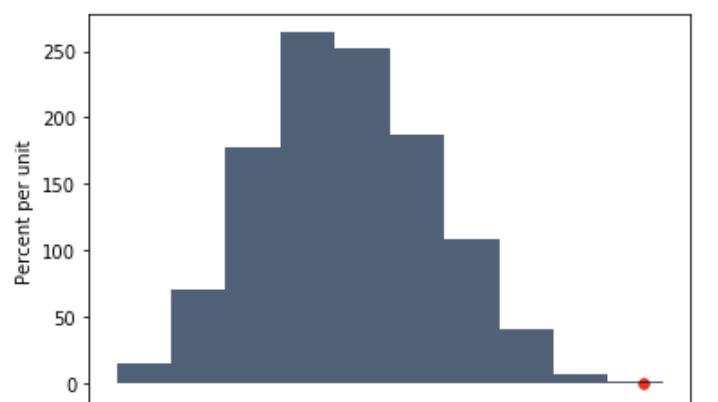
\includegraphics[scale=0.5]{statistics.png}
\end{center}\\
\\ 
\subq{2} Select the best conclusion from the options below: 
\begin{itemize}[label=\bubble]
\item Our data is more consistent with the null hypothesis.
\item Our data is more consistent with the alternative hypothesis.
\item It is impossible to decide given just the histogram above.
\end{itemize}
\solution{Option 2}
\end{enumerate}



